\documentclass{standalone}
\usepackage{tikz}

\begin{document}
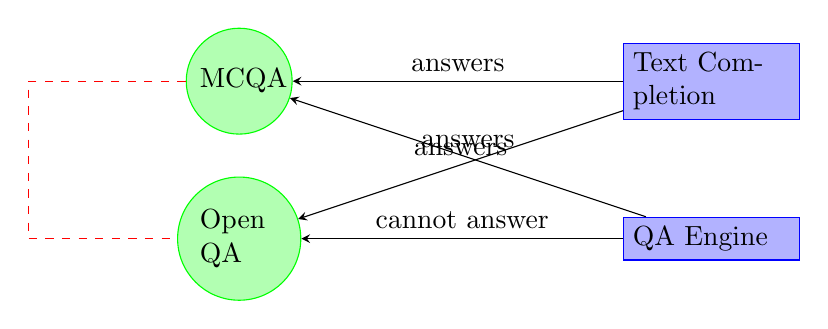
\begin{tikzpicture}[node distance=2cm]

    % Define styles for nodes
    \tikzset{
        dataset/.style={circle, draw=green, fill=green!30, text width=1cm},
        model/.style={rectangle, draw=blue, fill=blue!30, text width=2cm}
    }

    % Nodes representing datasets
    \node[dataset] (MCQA) {MCQA};
    \node[dataset] (OpenQA) [below of=MCQA] {Open QA};

    % Nodes representing models
    \node[model] (TextCompletion) [right of=MCQA, xshift=4cm] {Text Completion};
    \node[model] (QAE) [right of=OpenQA, xshift=4cm] {QA Engine};

    % Connections between models and datasets
    \draw[-stealth] (TextCompletion) -- node[above] {answers} (MCQA);
    \draw[-stealth] (TextCompletion) -- node[above] {answers} (OpenQA);
    \draw[-stealth] (QAE) -- node[above] {answers} (MCQA);
    \draw[-stealth] (QAE) -- node[above] {cannot answer} (OpenQA);

    % Indicating that MCQA can be converted to Open QA
    \draw[dashed, red] (MCQA.west) -- ++(-2,0) |- (OpenQA.west);

\end{tikzpicture}
\end{document}